\subsection{Herstellung mechanische Komponenten}
Die konzeptionellen CAD-Zeichnungen werden ab Semesterwoche 2 weiter 
ausgearbeitet, abgewickelt und die Fertigungszeichnungen erstellt. Hierbei 
müssen hauptsächlich Details wie Bohrungen für die Nieten angebracht und 
einige konstruktive Anpassungen vorgenommen werden. 
Ab Semesterwoche 3 können die ersten Teile an der Fräsmaschine im 
Elektrotechniklabor produziert werden, wobei parallel  hierzu die restlichen 
Komponenten am CAD fertiggestellt werden.  Um die gebogenen Innenkanten der 
Aussparungen zu realisieren, werden die gefrästen Blechteile mit einer 
Handpresse und eigens hierfür hergestellten Werkzeugen gefertigt.
In Semesterwoche 4 wird die Grundplatte zur Fertigung an der HSLU in Auftrag 
gegeben.
In Semesterwoche 5 werden zusätzlich einige Teile zum spanenden Herstellen, 
sowie zum 3D-Drucken in Auftrag gegeben. Ebenfalls wird eine 
Rohmaterialbestellung aufgegeben.
Die in Auftrag gegebenen Teile können in Semesterwoche 6 abgeholt werden, 
wobei das  Rohmaterial fälschlicherweise aus Stahl, anstatt aus Aluminium, 
bestellt wurde. Eine neue Bestellung des richtigen Rohmaterials wird abgesetzt.
In Semesterwoche 7 können die bestellten Teile, sowie die zum Biegen extern in 
Auftrag gegebenen Teile abgeholt werden. Des Weiteren wird mit dem Zusammenbau 
der einzelnen Komponenten begonnen. Aufgrund eines beim Biegen entstandenen 
Verzugs einzelner Bauteile und einiger konstruktiver Ungenauigkeiten müssen 
diverse Bohrungen durch feilen nachgebessert werden. Durch Niethefter kann die 
Konstruktion bis zum endgültigen Vernieten aufgebaut werden.

\begin{figure}[h!]
	\centering
	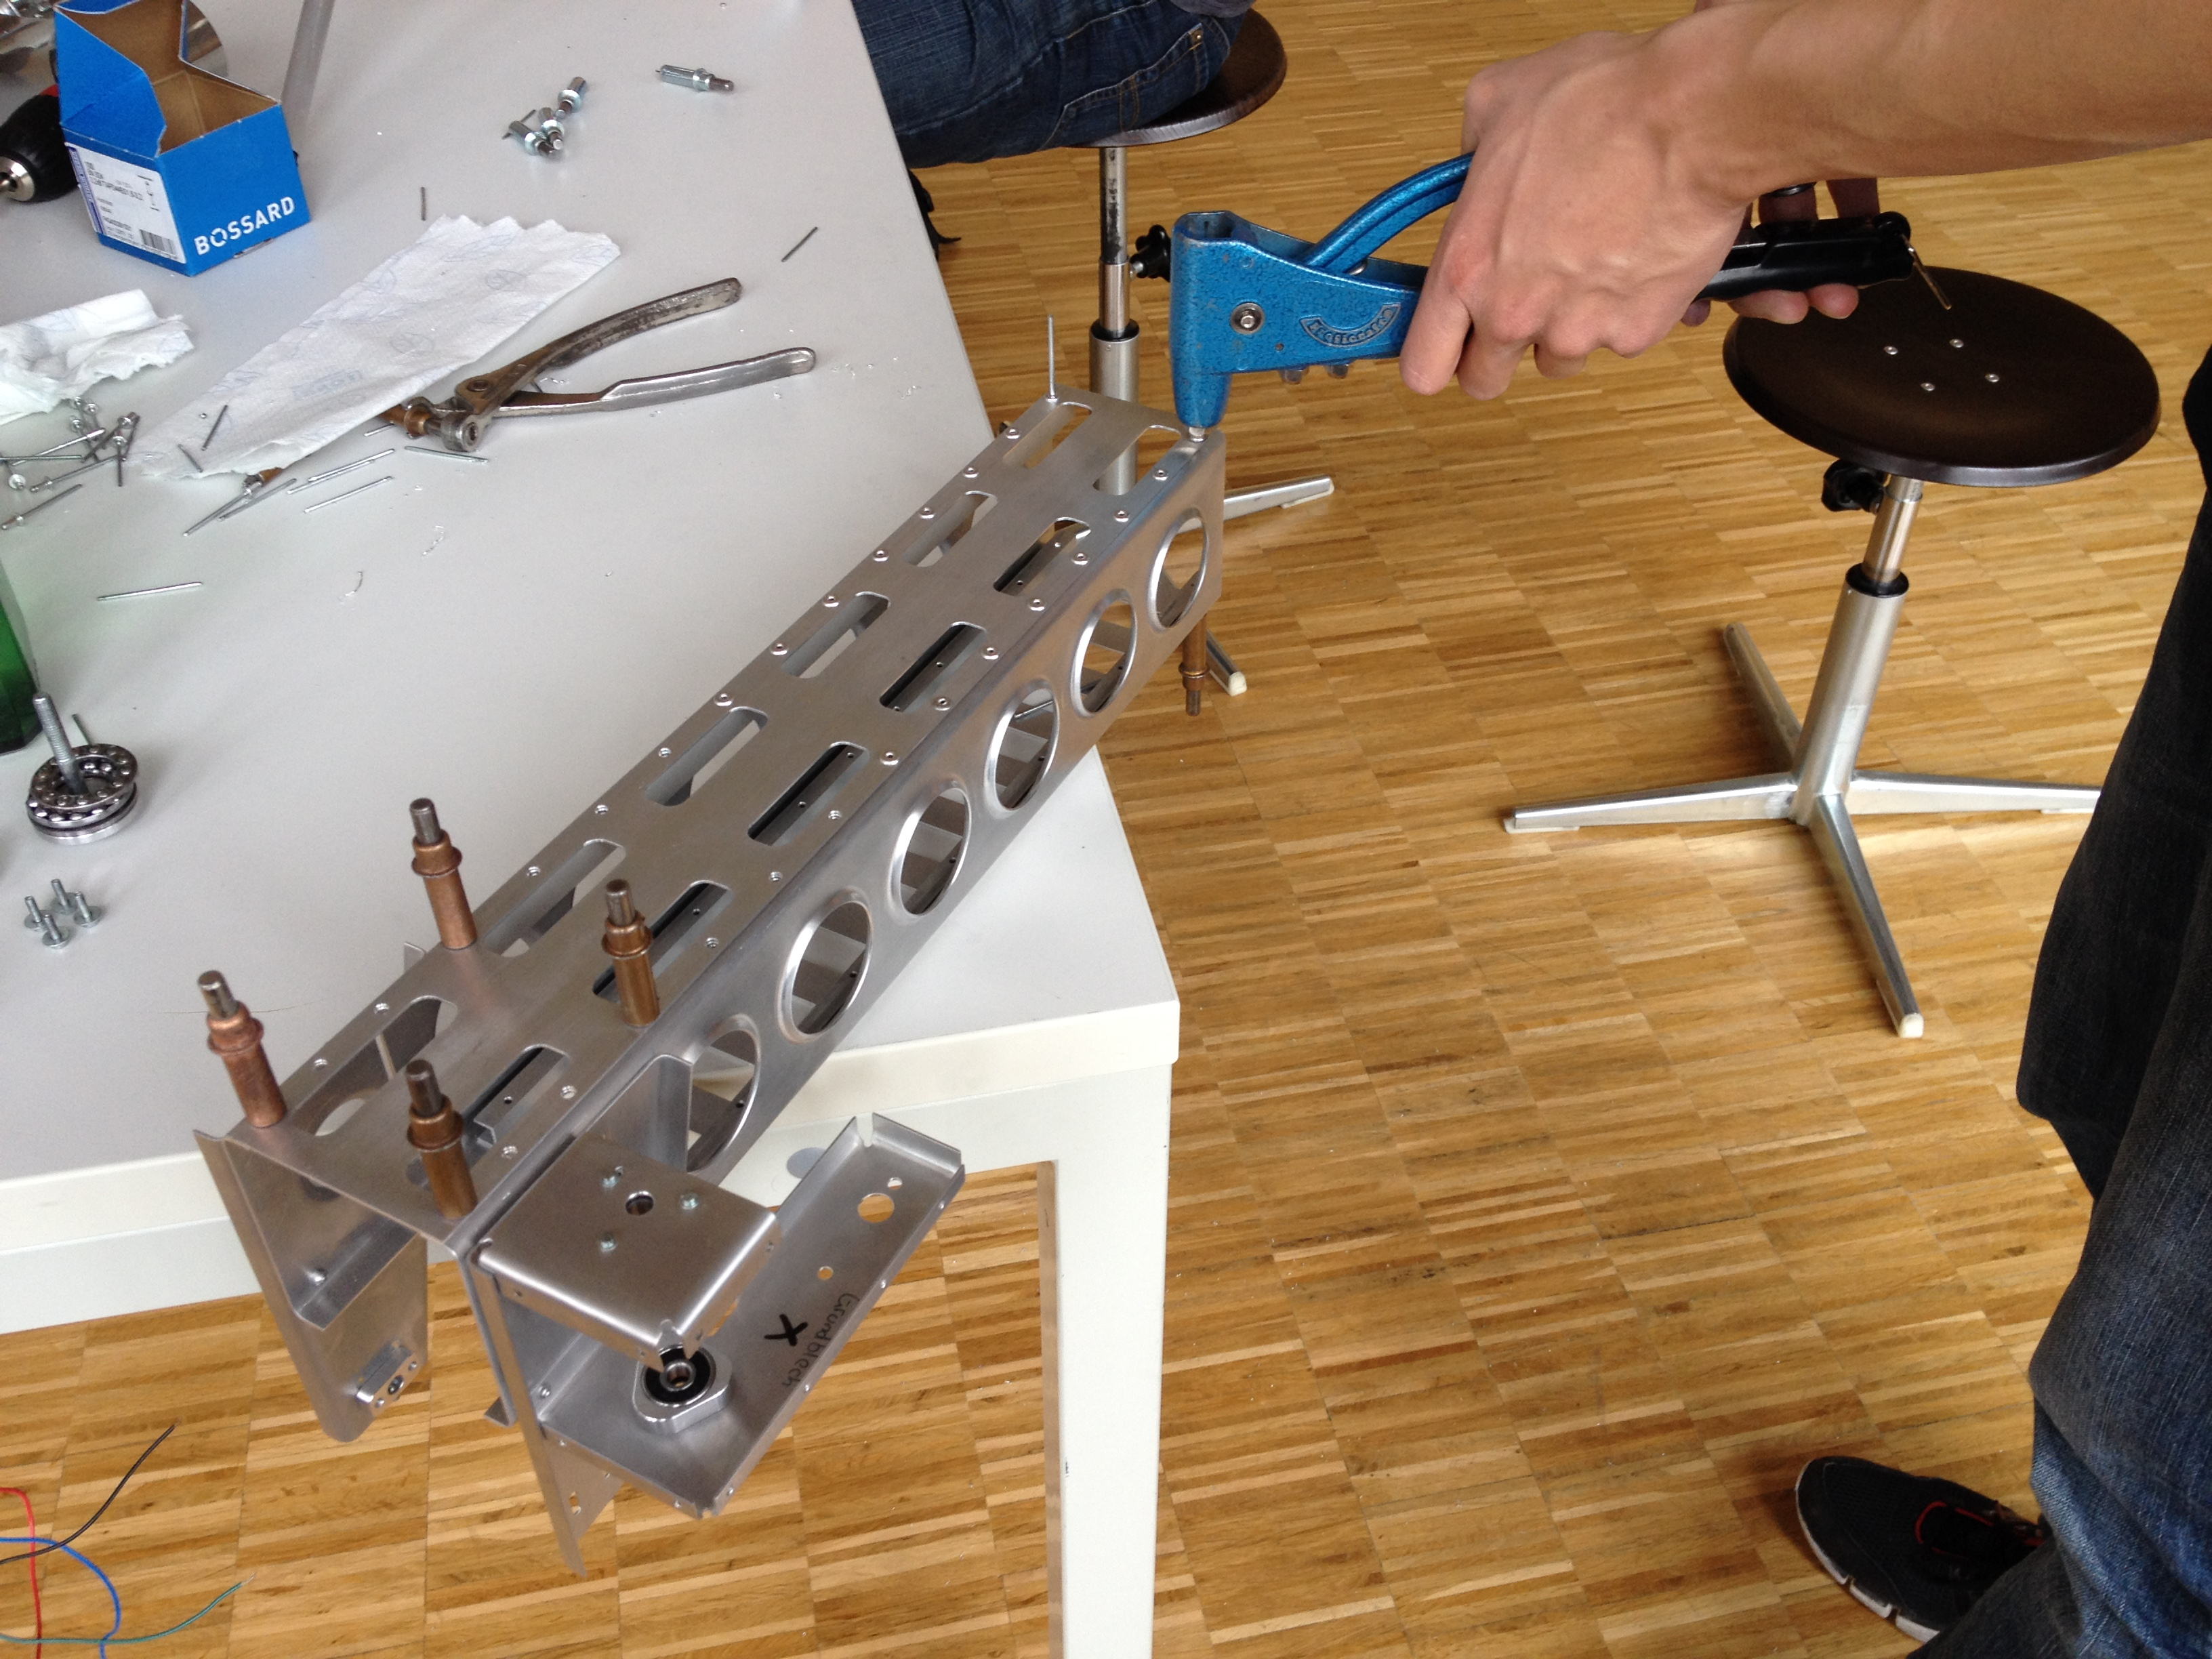
\includegraphics[width=0.5\textwidth]{fig/IMG_2290.JPG}
	\caption{Zusammenbau Balllager}
	\label{fig:Zusammenbau Balllager}
\end{figure}

\begin{figure}[h!]
	\centering
	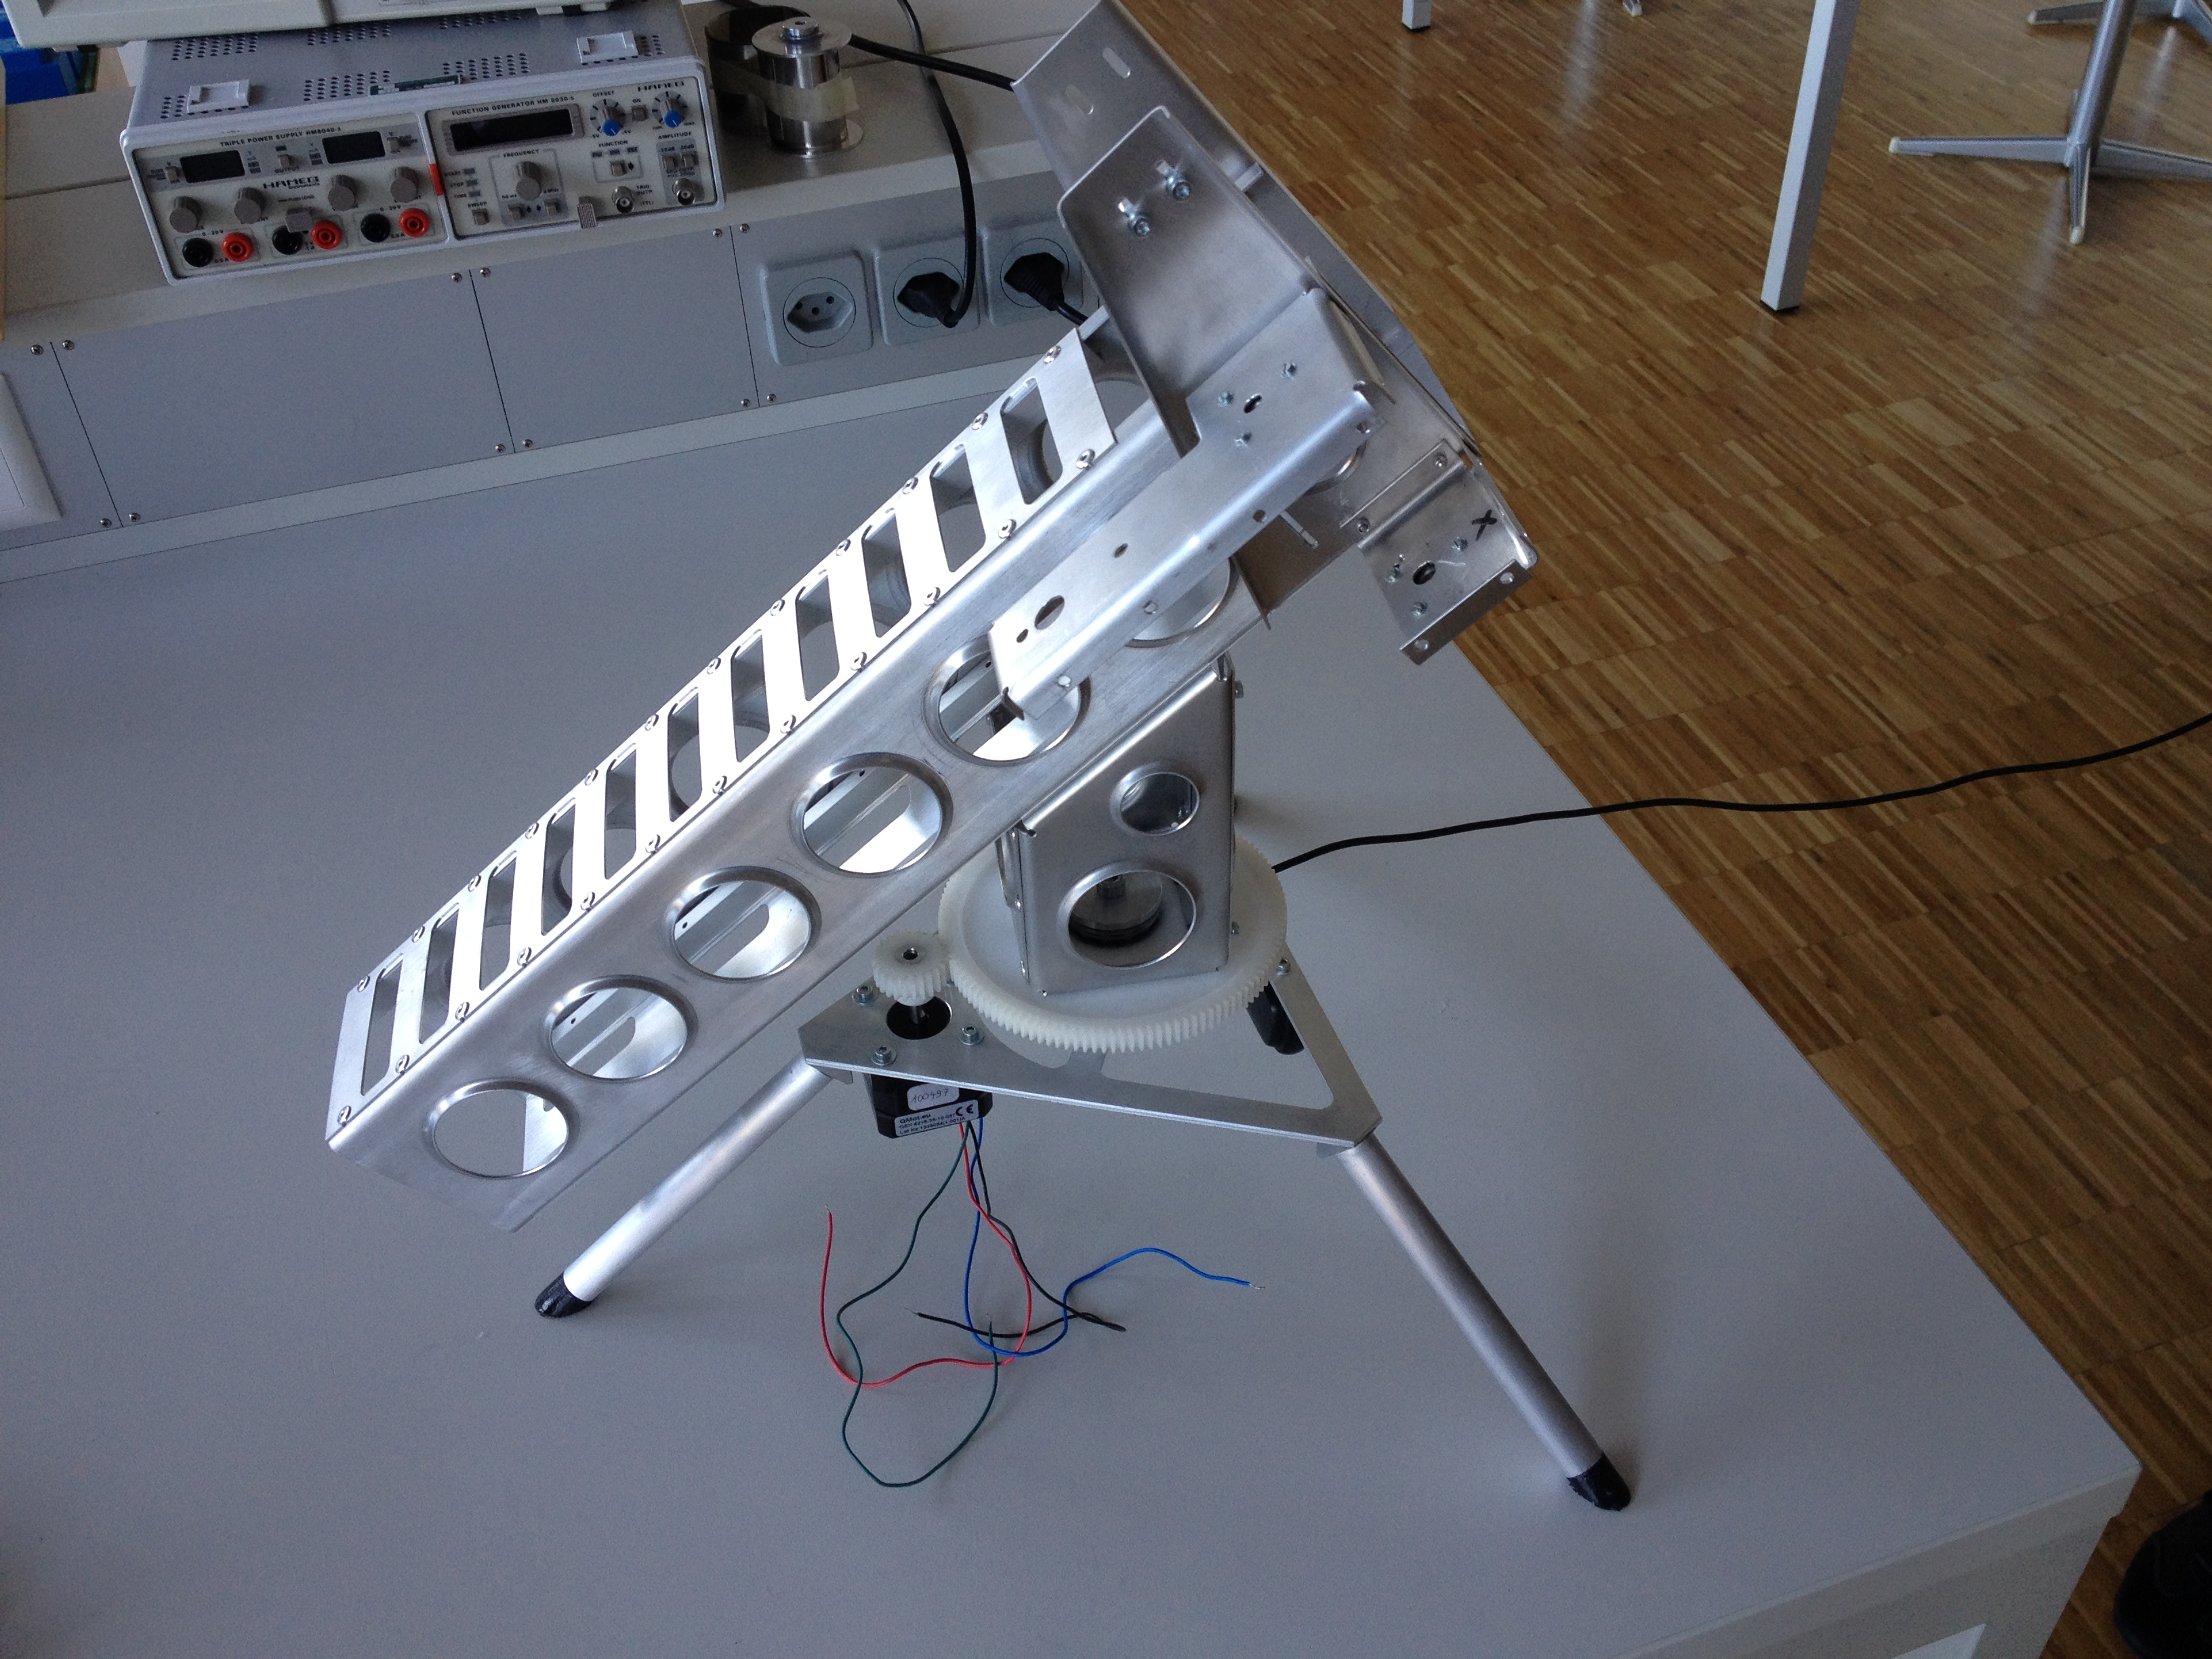
\includegraphics[width=0.5\textwidth]{fig/IMG_2303.JPG}
	\caption{Unvollständiger Aufbau}
	\label{fig:Unvollständiger Aufbau}
\end{figure}
\FloatBarrier

\subsubsection{Motor}
Zunächst wird der Rotor des Motors auf einer CNC-Fräse gefräst und der 
Stahlring eingepresst. Anschliessend werden sämtliche Magnete von Hand 
eingesetzt und mit Zweikomponentenklebstoff befestigt. Die Statorbleche für 
den Motor stammen aus Floppydisk-Laufwerken. Dazu müssen, für einen Motor, die 
Statoren aus zwei Laufwerken ausgebaut werden. Anschliessend werden die 
bestehenden Wicklungen von den Statoren entfernt. Die Statorbleche und die 
Kunststoffisolatoren werden für den neuen Motor weiterverwendet. Dazu werden 
die Statorbleche aus zwei Motoren aufeinandergelegt und mit der Halterung 
verschraubt. Anschliessend wird der Stator mit neuem Kupferlackdraht 
bewickelt. Nach dem Bewickeln und fixieren der Wicklungen wird der Stator 
passend auf den Durchmesser des Rotors abgedreht. Danach kann der Stator auf 
der passenden Aufnahme befestigt und der Motor zusammengesetzt werden. Der 
Pneu wird für einen guten Sitz auf der Aluminiumfelge passend ausgedreht. 
\begin{figure}[h!]
    \begin{center}
        \begin{minipage}[c]{0.25\textwidth}
            \begin{subfigure}[a]{\textwidth}
                \includegraphics[width=1.0\textwidth, trim=800 200 900 650, clip=true]{fig/DSC02759.JPG}
                \caption{Laufwerkmotor \\ $\qquad$}
                \label{m_motor_stator_before}
            \end{subfigure}
        \end{minipage}
        \begin{minipage}[c]{0.05\textwidth}
            \Huge$\Rightarrow$
        \end{minipage}
        \begin{minipage}[c]{0.25\textwidth}
            \begin{subfigure}[a]{\textwidth}
                \includegraphics[width=1.0\textwidth, trim=600 200 600 200, clip=true]{fig/DSC02940.JPG}
                \caption{unbewickelter Stator \\ $\qquad$}
                \label{m_motor_stator_empty}
            \end{subfigure}
        \end{minipage}
        \begin{minipage}[c]{0.05\textwidth}
            \Huge$\Rightarrow$
        \end{minipage}
        \begin{minipage}[c]{0.25\textwidth}
            \begin{subfigure}[a]{\textwidth}
                \includegraphics[width=1.0\textwidth, trim=500 100 500 100, clip=true]{fig/DSC02756.JPG}
                \caption{Motor mit bewickeltem Stator}
                \label{m_motor_stator_finished}
            \end{subfigure}
        \end{minipage}
    \end{center}
    \caption{Herstellung des Stators}
    \label{m_motor_stator}
\end{figure}
\FloatBarrier

\clearpage
\paragraph{Nachfolgend werden die speziellen Anpassungen einzelner Komponenten genauer beschrieben:}

\paragraph{Balllager}
Anhand der Erfahrungen erster Testläufe wird entschieden, dass keine 
Verstärkung an der Unterseite des vorderen Endes notwendig ist. Diese 
Verstärkung hätte eine zu starke Durchbiegung des Blechs beim 
Abschuss der Bälle verhindert.

\paragraph{Ballnachschub}
Beim Zusammenbau wird festgestellt, dass die Welle der Trommel einen zu 
grossen Durchmesser hat und daher mit Hilfe einer Handbohrmaschine und 
gewöhnlichem Schleifpapier auf das gewünschte Mass geschliffen werden muss.

\paragraph{Drehvorrichtung}
Um weiteres Gewicht einzusparen, wird die bereits hergestellte Grundplatte auf 
die halbe Höhe überfräst.

\begin{figure}[h!]
	\centering
	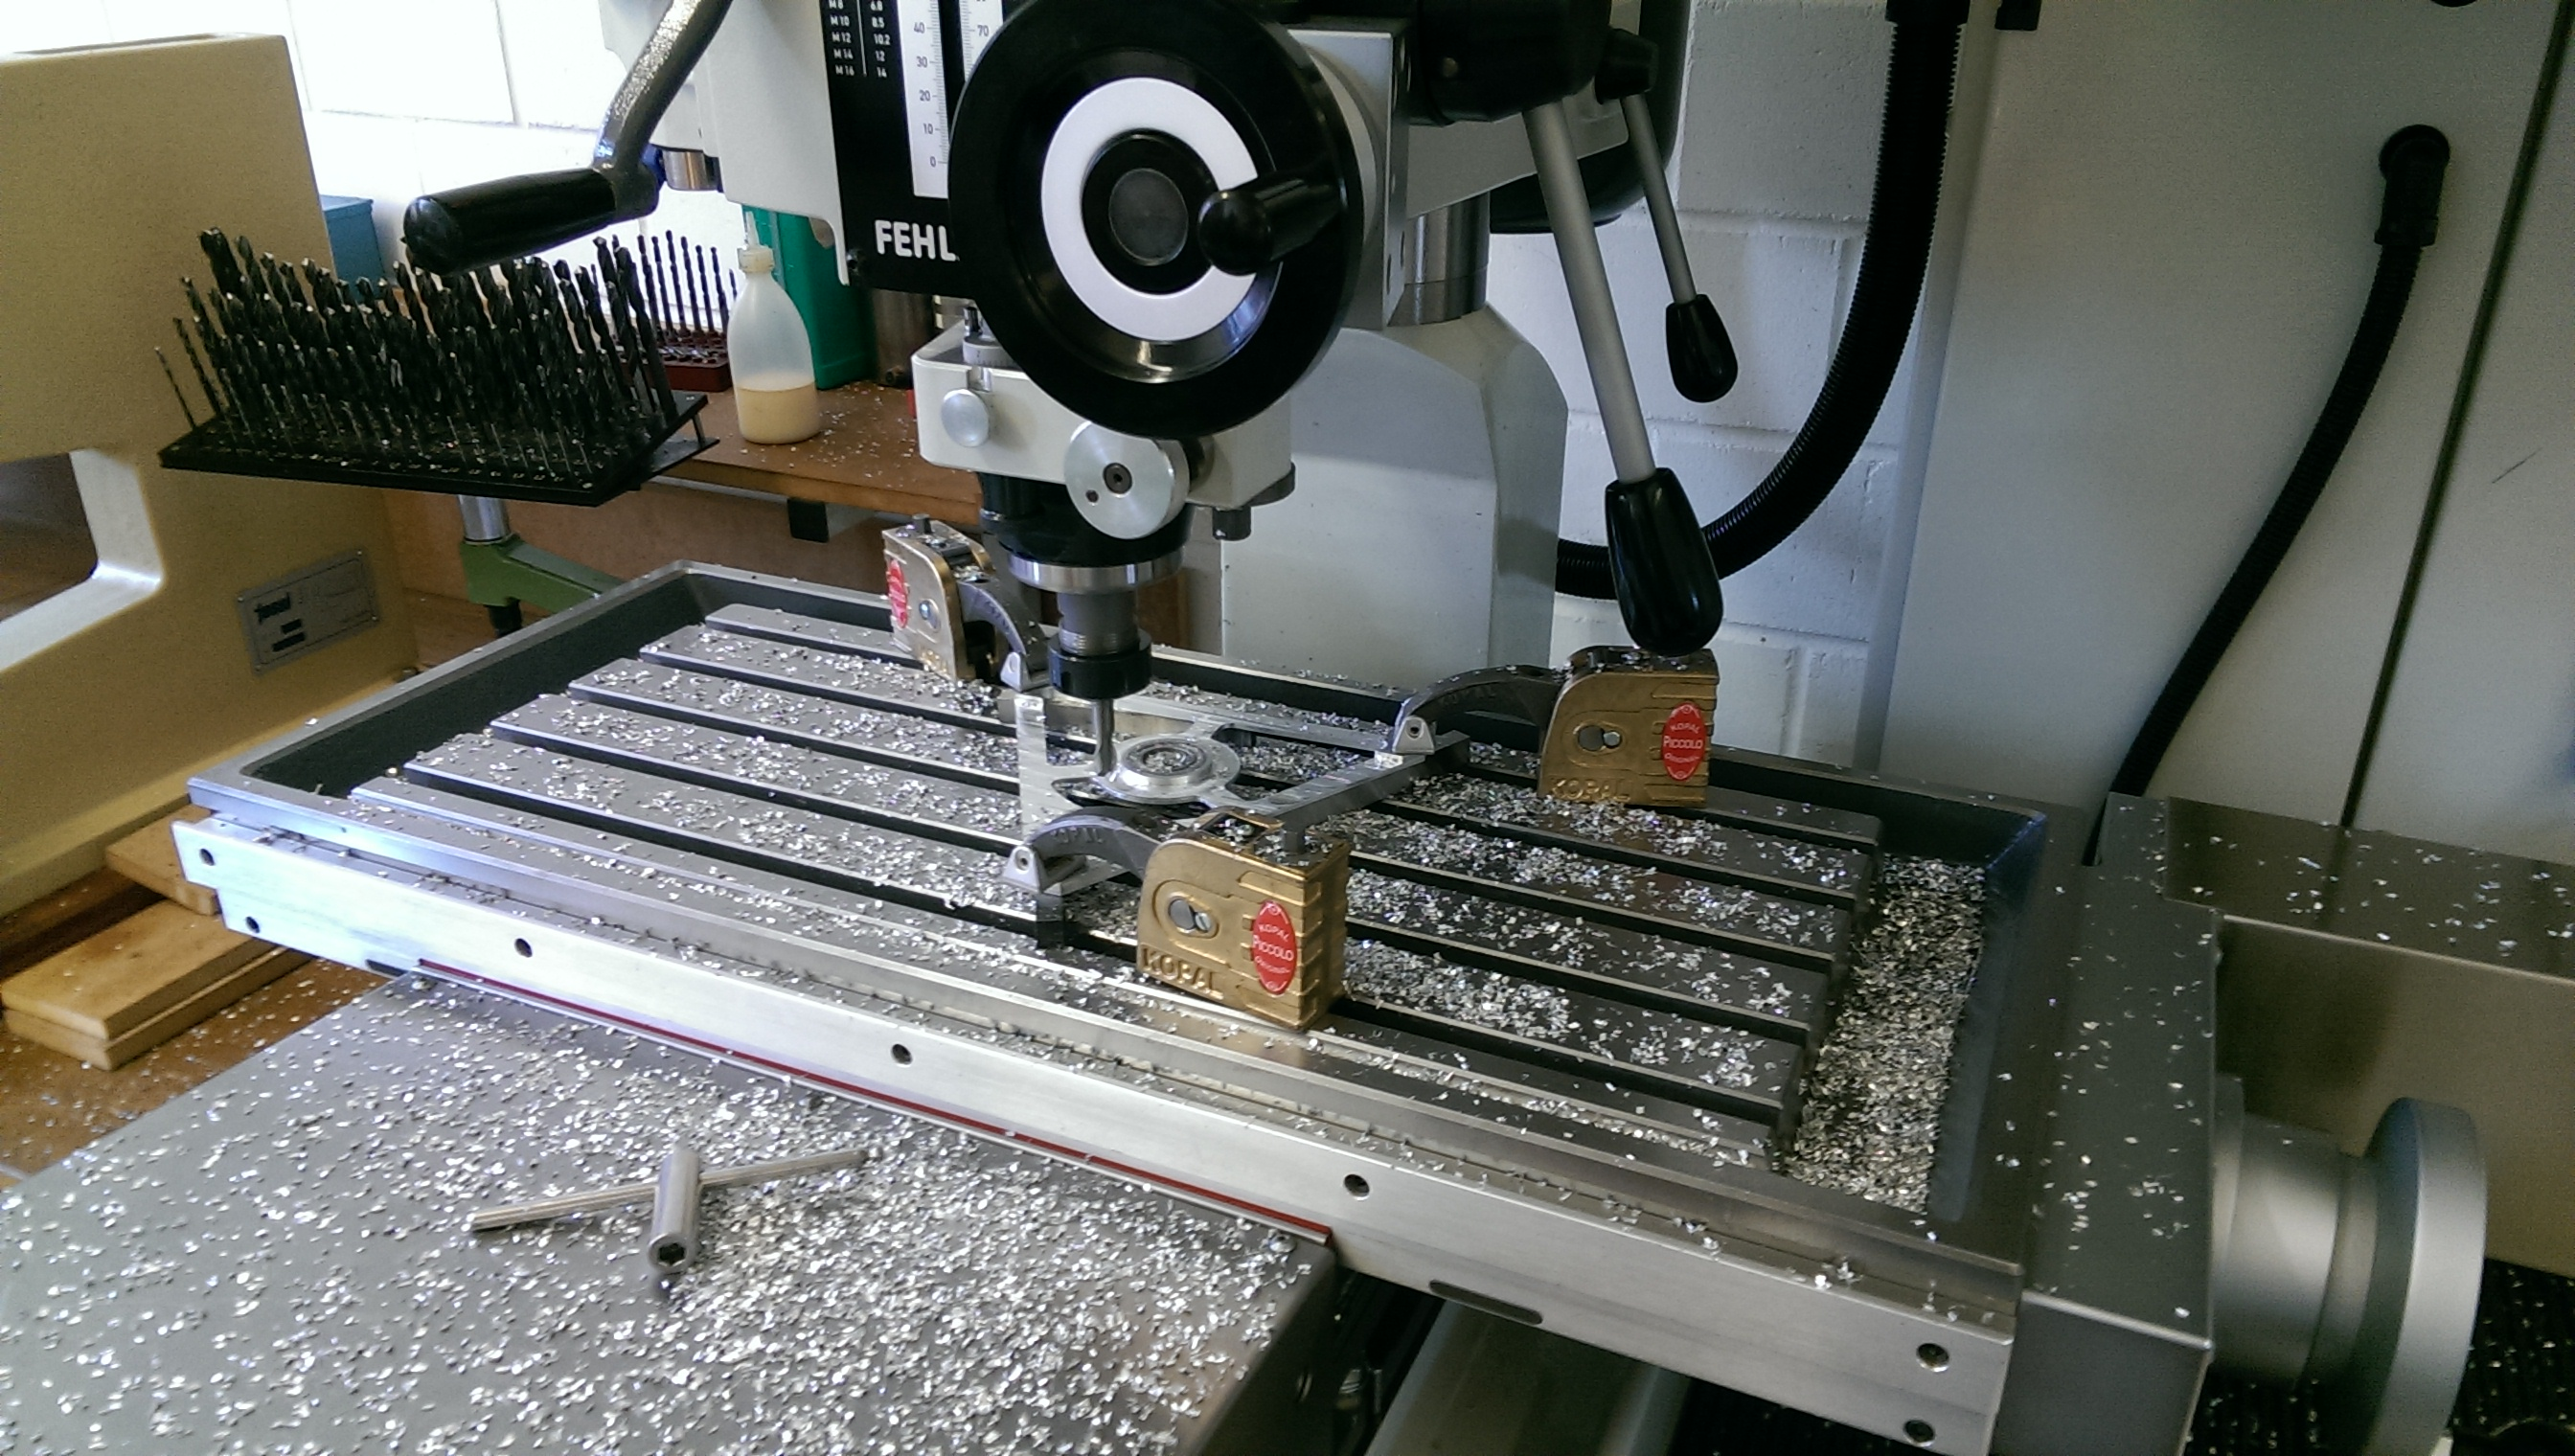
\includegraphics[width=0.5\textwidth]{fig/IMAG0357.jpg}
	\caption{Überfräsen der Grundplatte}
	\label{fig:Grundplatte fräsen}
\end{figure}
\FloatBarrier

\paragraph{Motorhalterung}
Beim Zusammenbau wird bemerkt, dass die Langlöcher der Motorenhalterung zu 
kurz ausgeführt wurden um einen guten Anpressdruck der Bälle zu ermöglichen. 
Daher werden diese durch feilen verlängert.

\paragraph{Turm}
Die Muttern der Wartungsklappe werden auf der Innenseite des Turms mit 
Zweikomponentenklebstoff angebracht. 

\begin{figure}[h!]
	\centering
	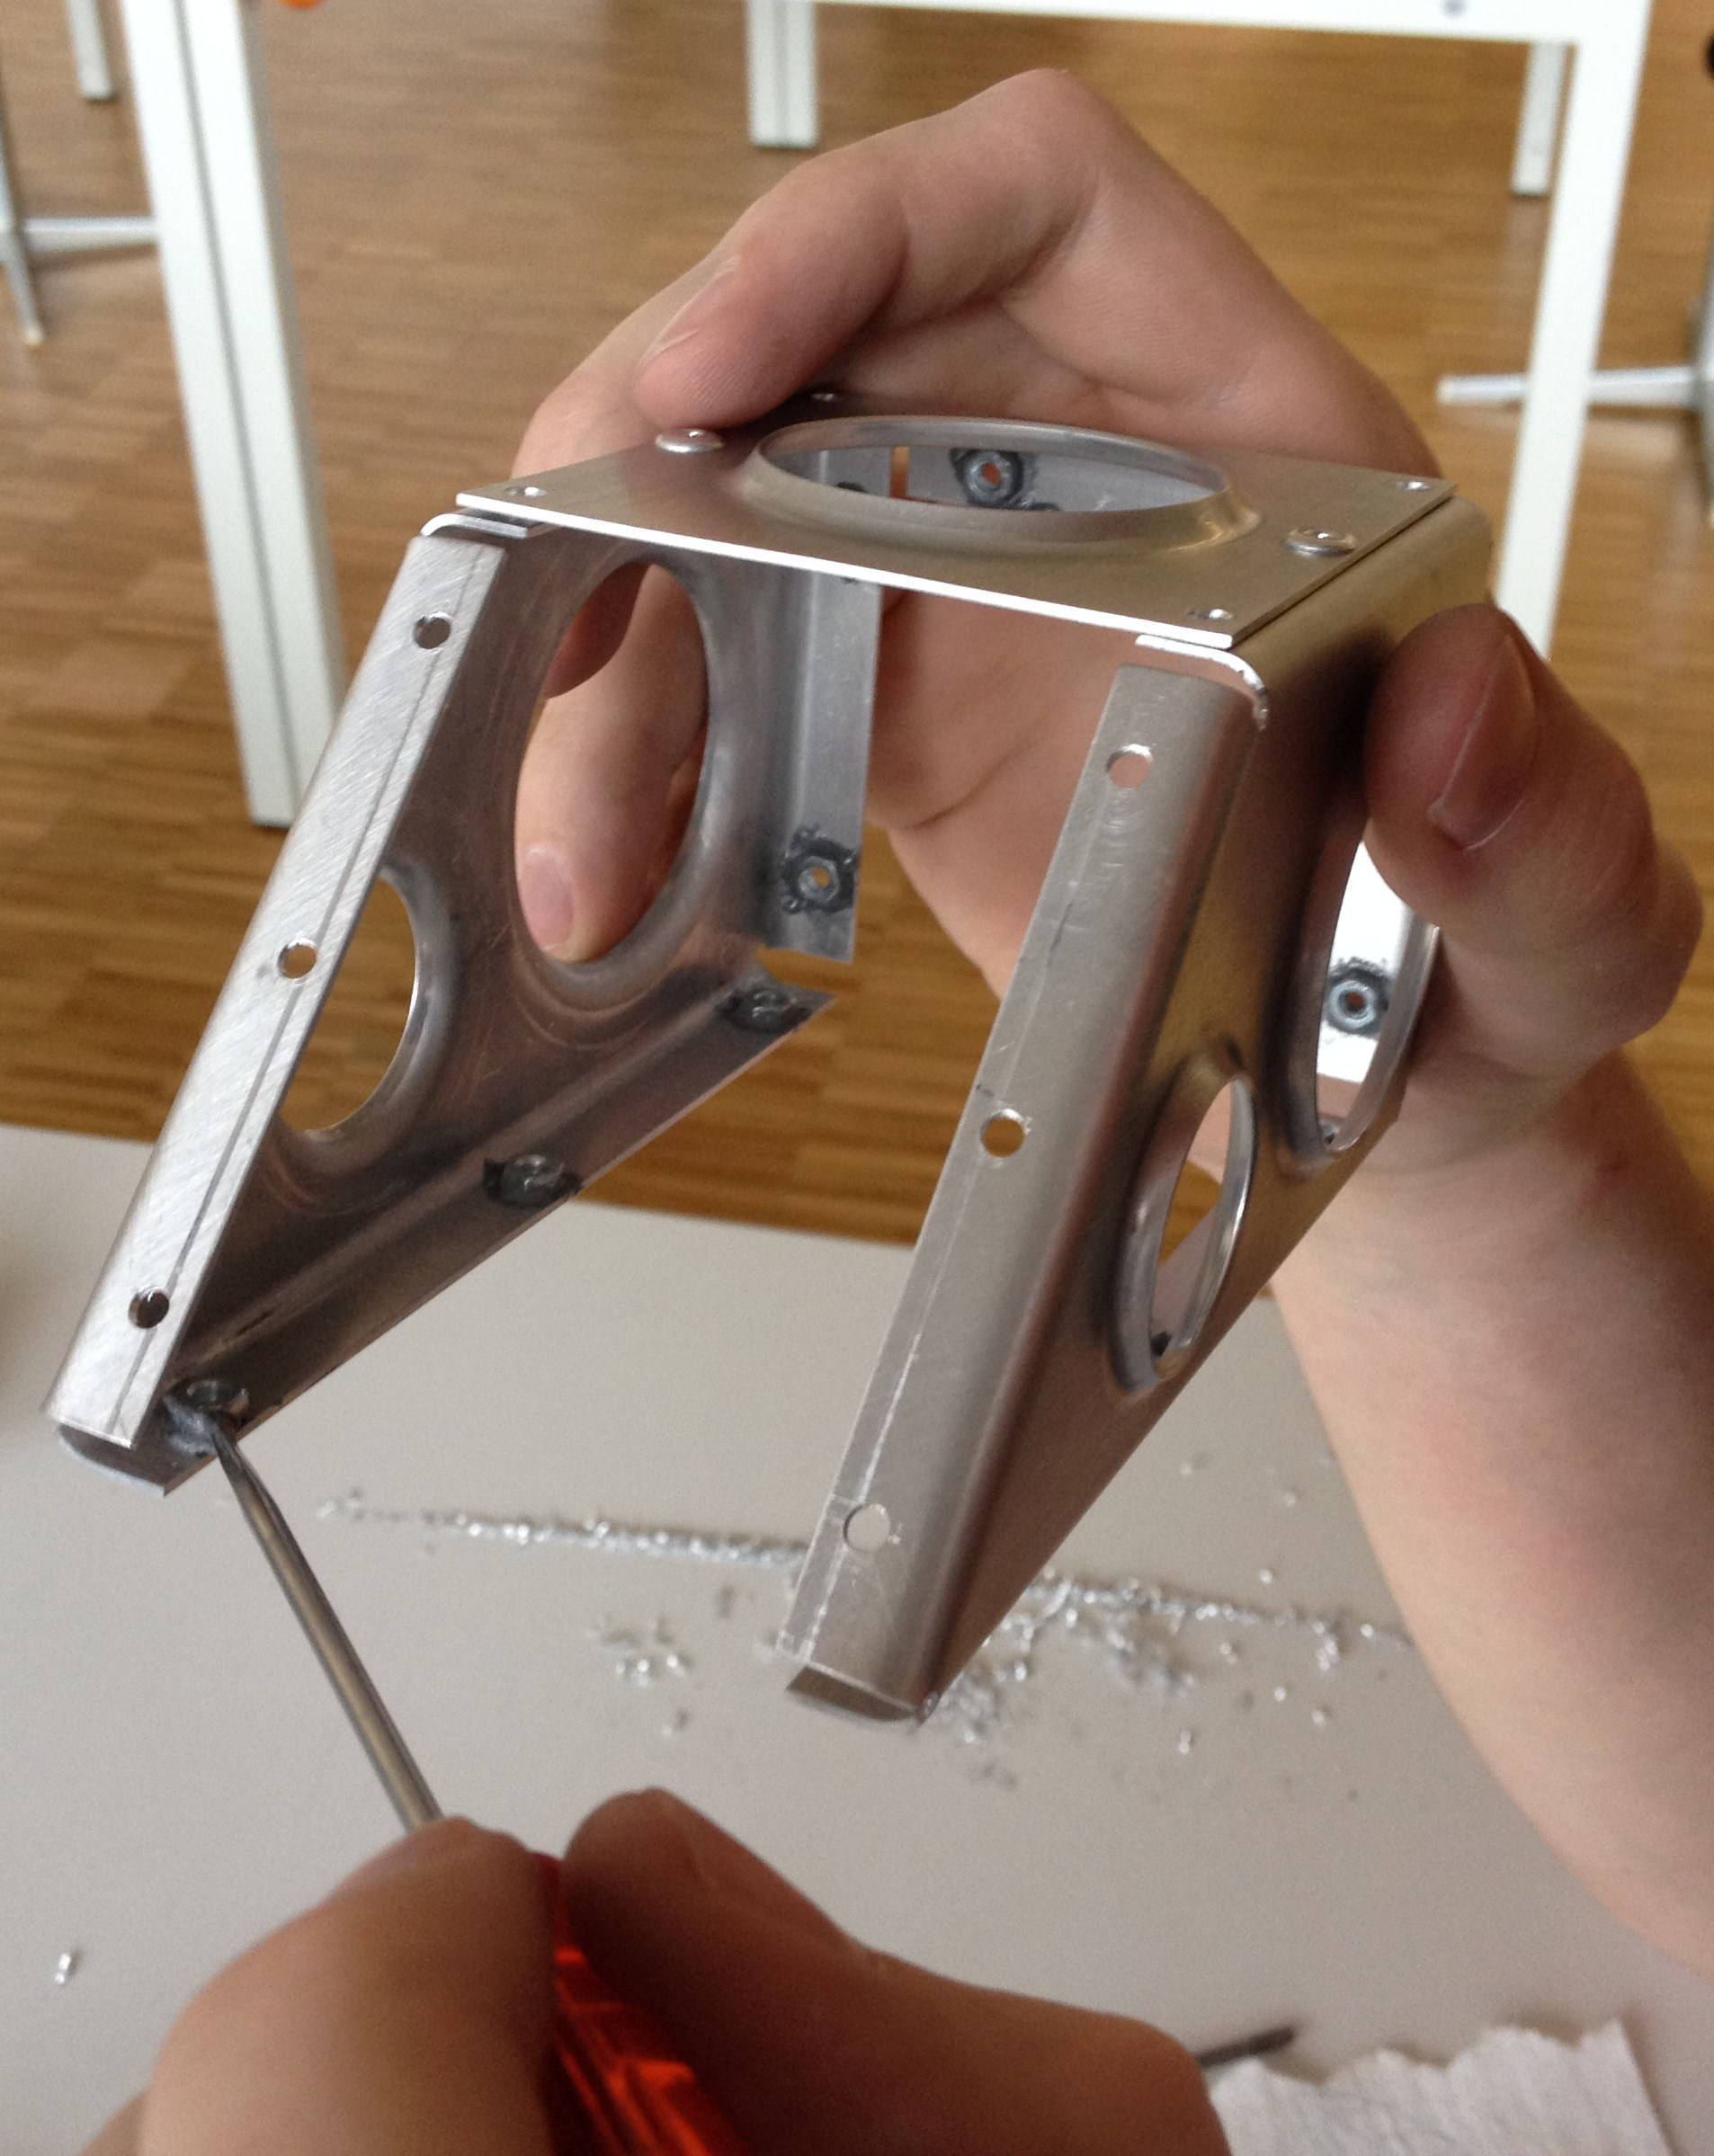
\includegraphics[width=0.3\textwidth, trim=0 100 0 100, clip=true]{fig/IMG_2292.JPG}
	\caption{Kleben der Muttern}
	\label{fig:Muttern Kleben}
\end{figure}
\FloatBarrier

